%
% Main document
% ===========================================================================
% This is part of the document "Project documentation template".
% Authors: brd3, kaa1
%

%---------------------------------------------------------------------------
\documentclass[
a4paper,					% paper format
10pt,							% fontsize
twoside,					% double-sided
openright,				% begin new chapter on right side
notitlepage,			% use no standard title page
parskip=half,			% set paragraph skip to half of a line
]{scrreprt}					% KOMA-script report
%---------------------------------------------------------------------------

\raggedbottom
\KOMAoptions{cleardoublepage=plain}			% Add header and footer on blank pages


% Load Standard Packages:
%---------------------------------------------------------------------------
\usepackage[standard-baselineskips]{cmbright}

\usepackage[english]{babel}										% english hyphenation
\usepackage{textcomp}													% additional symbols
\usepackage{ae}																% better resolution of Type1-Fonts 
\usepackage{fancyhdr}													% simple manipulation of header and footer 
\usepackage{etoolbox}													% color manipulation of header and footer
\usepackage{graphicx}                      		% integration of images
\usepackage{float}														% floating objects
\usepackage{caption}													% for captions of figures and tables
\usepackage{booktabs}													% package for nicer tables
\usepackage{tocvsec2}													% provides means of controlling the sectional numbering
\usepackage{listings}
\usepackage{inconsolata}
%\usepackage{tikz}
%\usepackage{pgf}
%\usepackage{pgfplots}
%\pgfplotsset{width=7cm,compat=1.16}
\usepackage{color}
\definecolor{lightgray}{rgb}{.9,.9,.9}
\definecolor{darkgray}{rgb}{.4,.4,.4}
\definecolor{purple}{rgb}{0.65, 0.12, 0.82}
\definecolor{bluekeywords}{rgb}{0.13,0.13,1}
\definecolor{greencomments}{rgb}{0,0.5,0}
\definecolor{redstrings}{rgb}{0.9,0,0}

\lstdefinelanguage{JavaScript}{
morekeywords={class, export, boolean, throw, implements, import, this, do, if, in, for, let, new, try, var, case, else, enum, eval, null, this, true, void, with, await, break, catch, class, const, false, super, throw, while, yield, delete, export, import, public, return, static, switch, typeof, default, extends, finally, package, private, continue, debugger, function, arguments, interface, protected, implements, instanceof},
sensitive=false,
comment=[l]{//},
morecomment=[s]{/*}{*/},
morestring=[b]{'},
morestring=[b]{"},
sensitive=true,
showspaces=false,
showtabs=false,
breaklines=true,
showstringspaces=false,
breakatwhitespace=true,
escapeinside={(*@}{@*)},
commentstyle=\color{greencomments},
keywordstyle=\color{bluekeywords},
stringstyle=\color{redstrings},
basicstyle=\ttfamily
}

\lstdefinelanguage{Go}{
morekeywords=[1]{break,case,chan,const,continue,default,defer,%
else,fallthrough,for,func,go,goto,if,import,interface,map,%
package,range,return,select,struct,switch,type,var},%keywords
morekeywords=[2]{append,cap,close,complex,copy,delete,imag,len,%
make,new,panic,print,println,real,recover},%functions
morekeywords=[3]{nil,true,false,iota}%constants
morekeywords=[4]{bool,byte,complex64,complex128,error,float32,%
float64,int,int8,int16,int32,int64,rune,string,uint,uint8,%
uint16,uint32,uint64,uintptr},%types
% Strings : "toto", 'toto', `toto`
morestring=[b]{"},
morestring=[b]{'},
morestring=[b]{`},
% Comments : /* comment */ and // comment
comment=[l]{//},
morecomment=[s]{/*}{*/},
% Options
sensitive=true,
showspaces=false,
showtabs=false,
breaklines=true,
showstringspaces=false,
breakatwhitespace=true,
escapeinside={(*@}{@*)},
commentstyle=\color{greencomments},
keywordstyle=\color{bluekeywords},
stringstyle=\color{redstrings},
basicstyle=\ttfamily
}

%---------------------------------------------------------------------------

% Load Math Packages
%---------------------------------------------------------------------------
\usepackage{amsmath}                    	   	% various features to facilitate writing math formulas
\usepackage{amsthm}                       	 	% enhanced version of latex's newtheorem
\usepackage{amsfonts}                      		% set of miscellaneous TeX fonts that augment the standard CM
\usepackage{amssymb}													% mathematical special characters
\usepackage{exscale}													% mathematical size corresponds to textsize
%---------------------------------------------------------------------------

% Package to facilitate placement of boxes at absolute positions
%---------------------------------------------------------------------------
\usepackage[absolute]{textpos}
\setlength{\TPHorizModule}{1mm}
\setlength{\TPVertModule}{1mm}
%---------------------------------------------------------------------------					

% Definition of Colors
%---------------------------------------------------------------------------
\definecolor{linkblue}{rgb}{0,0,0.8}            % Standard
\definecolor{darkblue}{rgb}{0,0.08,0.45}        % Dark blue
\definecolor{bfhgrey}{rgb}{0.41,0.49,0.57}      % BFH grey
%\definecolor{linkcolor}{rgb}{0,0,0.8}     			% Blue for the web- and cd-version!
\definecolor{linkcolor}{rgb}{0,0,0}        			% Black for the print-version!
%---------------------------------------------------------------------------

%---------------------------------------------------------------------------

% Set up page dimension
%---------------------------------------------------------------------------
\usepackage{geometry}
\geometry{
a4paper,
left=28mm,
right=15mm,
top=30mm,
headheight=20mm,
headsep=10mm,
textheight=242mm,
footskip=15mm
}
%---------------------------------------------------------------------------

% Makeindex Package
%---------------------------------------------------------------------------
\usepackage{makeidx}                         		% To produce index
\makeindex                                    	% Index-Initialisation
%---------------------------------------------------------------------------

% Glossary Package
%---------------------------------------------------------------------------
% the glossaries package uses makeindex
% if you use TeXnicCenter do the following steps:
%  - Goto "Ausgabeprofile definieren" (ctrl + F7)
%  - Select the profile "LaTeX => PDF"
%  - Add in register "Nachbearbeitung" a new "Postprozessoren" point named Glossar
%  - Select makeindex.exe in the field "Anwendung" ( ..\MiKTeX x.x\miktex\bin\makeindex.exe )
%  - Add this [ -s "%tm.ist" -t "%tm.glg" -o "%tm.gls" "%tm.glo" ] in the field "Argumente"
%
% for futher informations go to http://ewus.de/tipp-1029.html
%---------------------------------------------------------------------------
\usepackage[nonumberlist,acronym]{glossaries}

\newglossaryentry{BibTeX}{name={BibTeX},description={Program for the creation of 	bibliographical references and directories in \TeX or \LaTeX documents}}
\newglossaryentry{Index}{name={Index},description={Index with keywords from text}}




\newacronym{AAL2}{AAL2}{Authenticator Assurance Level 2}
\newacronym{AAL3}{AAL3}{Authenticator Assurance Level 3}
\newacronym{AAL}{AAL}{Authenticator Assurance Level}
\newacronym{AATL}{AATL}{Adobe Approved Trust List}
\newacronym{AES}{AES}{Advanced Electronic Signatures}
\newacronym{API}{API}{Application Programming Interface}
\newacronym{AVX2}{AVX2}{Advanced Vector Extensions 2}
\newacronym{BLS}{BLS}{Boneh-Lynn-Shacham}
\newacronym{CA}{CA}{Certificate Authority}
\newacronym{CAdES}{CAdES}{Cryptographic Message Syntax Advanced Electronic Signature}
\newacronym{CLR}{CLR}{.NET Common Language Runtime}
\newacronym{CMS}{CMS}{Cryptographic Message Syntax}
\newacronym{CORS}{CORS}{Cross-Origin Resource Sharing}
\newacronym{CRL}{CRL}{Certificate Revocation List}
\newacronym{CSC}{CSC}{Cloud Signature Consortium}
\newacronym{CSR}{CSR}{Certificate Signing Request}
\newacronym{CSRF}{CSRF}{Cross Site Request Forgery}
\newacronym{CSRNG}{CSRNG}{Cryptographically Secure Random Number Generator}
\newacronym{CSS}{CSS}{Cascading Stylesheets}
\newacronym{CT}{CT}{Certificate Transparency}
\newacronym{DER}{DER}{Distinguished Encoding Rules}
\newacronym{DNS}{DNS}{Domain Name System}
\newacronym{DoS}{DoS}{Denial of Service}
\newacronym{DSA}{DSA}{Digital Signature Algorithm}
\newacronym{DSS}{DSS}{Digital Signature Service}
\newacronym{ECC}{ECC}{Elliptic Curve Cryptography}
\newacronym{ECDSA}{ECDSA}{Elliptic Curve Digital Signature Algorithm}
\newacronym{Ed25519}{Ed25519}{EdDSA with Curve25519 and SHA-512}
\newacronym{EdDSA}{EdDSA}{Edwards-curved Digital Signature Algorithm}
\newacronym{eIDAS}{eIDAS}{electronic IDentification, Authentication and trust Services}
\newacronym{ETSI}{ETSI}{European Telecommunications Standards Institute}
\newacronym{EU}{EU}{European Union}
\newacronym{EUTL}{EUTL}{European Union Trust List}
\newacronym{FIDO}{FIDO}{Fast IDentity Online}
\newacronym{GMT}{GMT}{Greenwich Median Time}
\newacronym{GNU}{GNU}{GNU's Not Unix}
\newacronym{GUI}{GUI}{Graphical User Interface}
\newacronym{HKDF}{HKDF}{HMAC-based Key Derivation Function}
\newacronym{HMAC}{HMAC}{Keyed-Hash Message Authentication Code}
\newacronym{HSM}{HSM}{Hardware Security Module}
\newacronym{HTML}{HTML}{Hypertext Markup Language}
\newacronym{HTTP}{HTTP}{Hypertext Transfer Protocol}
\newacronym{HTTPS}{HTTPS}{HTTP over TLS}
\newacronym{IAL3}{IAL3}{Identity Assurance Level 3}
\newacronym{IAL}{IAL}{Identity Assurance Level}
\newacronym{ICT}{ICT}{Information and Communications Technologies}
\newacronym{IDE}{IDE}{Integrated Development Environment}
\newacronym{IDM}{IDM}{Identity and Access Management}
\newacronym{IDP}{IDP}{Identity Provider}
\newacronym{IEC}{IEC}{International Electrotechnical Commission}
\newacronym{IETF}{IETF}{Internet Engineering Task Force}
\newacronym{ISO}{ISO}{International Standards Organisation}
\newacronym{JKS}{JKS}{Java Keystore}
\newacronym{JSON}{JSON}{JavaScript Object Notation}
\newacronym{JVM}{JVM}{Java Virtual Machine}
\newacronym{JWK}{JWK}{JSON Web Key}
\newacronym{JWKS}{JWKS}{JSON Web Key Store}
\newacronym{JWS}{JWS}{JSON Web Signature}
\newacronym{JWT}{JWT}{JSON Web Token}
\newacronym{LoA}{LoA}{Level of assurance}
\newacronym{LTV}{LTV}{Long-Term Validation}
\newacronym{MAC}{MAC}{Message Authentication Code}
\newacronym{MFA}{MFA}{Multi-factor authentication}
\newacronym{NIST}{NIST}{National Institute of Standards and Technology}
\newacronym{OASIS}{OASIS}{Organisation for the Advancement of Structured Information Standards}
\newacronym{OCSP}{OCSP}{Online Certificate Status Protocol}
\newacronym{OIDC}{OIDC}{OpenID Connect}
\newacronym{OpenAPI}{OpenAPI}{Open Application Programming Interface}
\newacronym{PAdES}{PAdES}{Portable Document Format Advanced Electronic Signature}
\newacronym{PDF}{PDF}{Portable Document Format}
\newacronym{PEM}{PEM}{Privacy-Enhanced Mail}
\newacronym{PIN}{PIN}{Personal Identification Number}
\newacronym{PKCS7}{PKCS7}{Public Key Cryptography Standard 7}
\newacronym{PKCS10}{PKCS10}{Public Key Cryptography Standard 10}
\newacronym{PKCS}{PKCS}{Public Key Cryptography Standard}
\newacronym{PKI}{PKI}{Public Key Infrastructure}
\newacronym{PKS12}{PKS12}{Public-Key Cryptograpy Standards}
\newacronym{POC}{POC}{Proof Of Concept}
\newacronym{POJOs}{POJOs}{Plain old Java object}
\newacronym{PSS}{PSS}{Probabilistic Signature Scheme}
\newacronym{QES}{QES}{Qualified Electronic Signatures}
\newacronym{RA}{RA}{Registration Authority}
\newacronym{REST}{REST}{Representational State Transfer}
\newacronym{RFC}{RFC}{Request For Comments}
\newacronym{RNG}{RNG}{Random Number Generator}
\newacronym{RSA-PSS}{RSA-PSS}{RSA Probabilistic Signature Scheme}
\newacronym{RSA}{RSA}{Rivest-Shamir-Adleman}
\newacronym{SAD}{SAD}{Signature activation data}
\newacronym{SDK}{SDK}{Software Development Kit}
\newacronym{SHA-256}{SHA-256}{Secure Hash Algorithm 2 with 256-bit output length}
\newacronym{SHA-2}{SHA-2}{Secure Hash Algorithm 2}
\newacronym{SHA}{SHA}{Secure Hash Algorithm}
\newacronym{SIM}{SIM}{Subscriber Identity Module}
\newacronym{SMS}{SMS}{Short Message System}
\newacronym{SOAP}{SOAP}{Simple Object Access Protocol}
\newacronym{SPA}{SPA}{Single Page Application}
\newacronym{TLS}{TLS}{Transport Layer Security}
\newacronym{TOTP}{TOTP}{Time-based One Time Password}
\newacronym{TSA}{TSA}{Time Stamping Authority}
\newacronym{TSS}{TSS}{Timestamping Service}
\newacronym{UI}{UI}{User Interface}
\newacronym{UML}{UML}{Unified Modeling Language}
\newacronym{URI}{URI}{Unique Resource Identifier}
\newacronym{USB}{USB}{Universal Serial Bus}
\newacronym{VM}{VM}{Virtual Machine}
\newacronym{WASM}{WASM}{WebAssembly}
\newacronym{XAdES}{XAdES}{XML Advanced Electronic Signatures}
\newacronym{XML}{XML}{Extensible Markup Language}
\newacronym{BFH}{BFH}{Bern University of Applied Sciences}
\newacronym{SLF4J}{SLF4J}{Simple Logging Facade for Java}
\newacronym{CIO}{CIO}{Coroutine-based I/O}
\newacronym{TSP}{TSP}{Time-stamp Protocol}
\newacronym{DOM}{DOM}{Document Object Model}
\newacronym{FSF}{FSF}{Free Software Foundation}
\newacronym{JAR}{JAR}{Java Archive}
\newacronym{JRE}{JRE}{Java Runtime Environment}
\newacronym{JS}{JS}{JavaScript}
\newacronym{DI}{DI}{Dependency Injection}
\newacronym{CI}{CI}{Continuous Integration}
\newacronym{JOSE}{JOSE}{JavaScript Object Signing and Encryption}
\newacronym{VCS}{VCS}{Version Control System}
\newacronym{URL}{URL}{Uniform Resource Locator}

\makeglossaries
% Hyperref Package (Create links in a pdf)
%---------------------------------------------------------------------------
\usepackage[
pdftex,ngerman,bookmarks,plainpages=false,pdfpagelabels,
backref = {false},										% No index backreference
colorlinks = {true},                  % Color links in a PDF
hypertexnames = {true},               % no failures "same page(i)"
bookmarksopen = {true},               % opens the bar on the left side
bookmarksopenlevel = {0},             % depth of opened bookmarks
pdftitle = {Remote Signing Service},	   	% PDF-property
pdfauthor = {brd3},        					  % PDF-property
pdfsubject = {LaTeX Template},        % PDF-property
linkcolor = {linkcolor},              % Color of Links
citecolor = {linkcolor},              % Color of Cite-Links
urlcolor = {linkcolor},               % Color of URLs
]{hyperref}
%---------------------------------------------------------------------------

% Intro:
%---------------------------------------------------------------------------
\begin{document}                              	% Start Document
    \settocdepth{section}														% Set depth of toc
    \pagenumbering{roman}
    %---------------------------------------------------------------------------

    \providecommand{\heading}{Remote Signing Service}		%  Insert Title of Thesis here					% Titel der Arbeit aus Datei titel.tex lesen
    \providecommand{\versionnumber}{13.3.7}			%  Hier die aktuelle Versionsnummer eingeben
\providecommand{\versiondate}{\today}		%  Hier das Datum der aktuellen Version eingeben				% Versionsnummer und -datum aus Datei version.tex lesen

    % Set up header and footer
    %---------------------------------------------------------------------------
    \makeatletter
    \patchcmd{\@fancyhead}{\rlap}{\color{bfhgrey}\rlap}{}{}		% new color of header
    \patchcmd{\@fancyfoot}{\rlap}{\color{bfhgrey}\rlap}{}{}		% new color of footer
    \makeatother

    \fancyhf{}																		% clean all fields
    \fancypagestyle{plain}{												% new definition of plain style
    \fancyfoot[OR,EL]{\footnotesize \thepage} 	% footer right part --> page number
    \fancyfoot[OL,ER]{\footnotesize \heading, Version \versionnumber, \versiondate}	% footer even page left part
    }

    \renewcommand{\chaptermark}[1]{\markboth{\thechapter.  #1}{}}
    \renewcommand{\headrulewidth}{0pt}				% no header stripline
    \renewcommand{\footrulewidth}{0pt} 				% no bottom stripline

    \pagestyle{plain}
    %---------------------------------------------------------------------------


    % Title Page and Abstract
    %---------------------------------------------------------------------------
    %
% Project documentation template
% ===========================================================================
% This is part of the document "Project documentation template".
% Authors: brd3, kaa1
%

\begin{titlepage}


% BFH-Logo absolute placed at (28,12) on A4 and picture (16:9 or 15cm x 8.5cm)
% Actually not a realy satisfactory solution but working.
%---------------------------------------------------------------------------
\setlength{\unitlength}{1mm}
\begin{textblock}{20}[0,0](28,12)
	
\includegraphics[scale=1.0]{images/BFH_Logo_B.png}
\end{textblock}

% Institution / titel / subtitel / authors / experts:
%---------------------------------------------------------------------------
\begin{flushleft}

\vspace*{21mm}

\fontsize{26pt}{40pt}\selectfont 
\heading				\\							% Read heading from file leader/title.tex
\vspace{2mm}

\fontsize{16pt}{24pt}\selectfont\vspace{0.3em}
Accessible Electronic Signatures for Everybody 			\\				% Insert subheading
\vspace{5mm}

\fontsize{10pt}{12pt}\selectfont
\textbf{Bachelor Thesis by Gabor Tanz and Patrick Hirt} \\		% Insert text
\vspace{7mm}

% Abstract (eingeben):
%---------------------------------------------------------------------------
\begin{textblock}{150}(28,100)
\fontsize{10pt}{12pt}\selectfont
    TODO abstract TODO
\end{textblock}

\begin{textblock}{150}(28,225)
\fontsize{10pt}{17pt}\selectfont
\begin{tabbing}
xxxxxxxxxxxxxxx\=xxxxxxxxxxxxxxxxxxxxxxxxxxxxxxxxxxxxxxxxxxxxxxx \kill
Degree course:	\> [z.B. Electrical and Communication Engineering]	\\		% insert name of degree course
Authors:		\> [Test Peter, M\"uster R\"os\"a]		\\					% insert names
Tutor:	\> [Dr.~Xxxx Xxxx, Dr.~Yyyy Yyyy]		\\							% insert names
Constituent:	\> [Wwwww AG]					\\							% insert names
Experts:		\> [Dr.~Zzzz Zzzz]				\\							% insert names
Date:			\> \versiondate					\\							% read from file leader/version.tex
\end{tabbing}

\end{textblock}
\end{flushleft}

\begin{textblock}{150}(28,280)
\noindent 
\color{bfhgrey}\fontsize{9pt}{10pt}\selectfont
Berner Fachhochschule | Haute \'ecole sp\'ecialis\'ee bernoise | Bern University of Applied Sciences
\color{black}\selectfont
\end{textblock}


\end{titlepage}

%
% ===========================================================================
% EOF
%
		% activate for frontpage without picture
    %%
% Project documentation template
% ===========================================================================
% This is part of the document "Project documentation template".
% Authors: brd3, kaa1
%

\begin{titlepage}


% BFH-Logo absolute placed at (28,12) on A4 and picture (16:9 or 15cm x 8.5cm)
% Actually not a realy satisfactory solution but working.
%---------------------------------------------------------------------------
\setlength{\unitlength}{1mm}
\begin{textblock}{20}[0,0](28,12)
	
\includegraphics[scale=1.0]{images/BFH_Logo_B.png}
\end{textblock}

\begin{textblock}{154}(28,48)
	\begin{picture}(150,2)
		\put(0,0){\color{bfhgrey}\rule{150mm}{2mm}}
	\end{picture}
\end{textblock}

\begin{textblock}{154}[0,0](28,50)
	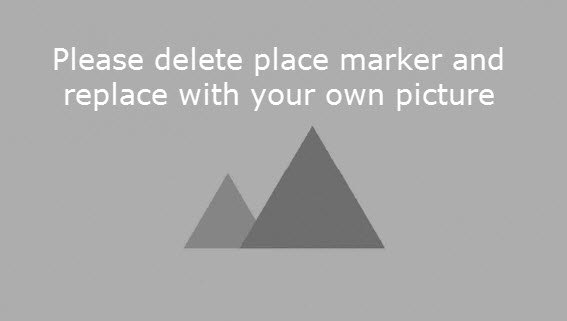
\includegraphics[scale=1.0]{images/placemarker.jpg}			% define cover picture
\end{textblock}

\begin{textblock}{154}(28,135)
	\begin{picture}(150,2)
		\put(0,0){\color{bfhgrey}\rule{150mm}{2mm}}
	\end{picture}
\end{textblock}
\color{black}

% Institution / titel / subtitel / authors / experts:
%---------------------------------------------------------------------------
\begin{flushleft}

\vspace*{115mm}

\fontsize{26pt}{28pt}\selectfont 
\heading				\\							% Read heading from file leader/title.tex
\vspace{2mm}

\fontsize{16pt}{20pt}\selectfont\vspace{0.3em}
Place your subheading here 			\\				% Insert subheading
\vspace{5mm}

\fontsize{10pt}{12pt}\selectfont
\textbf{Description of thesis (semester- / Bachelor thesis / etc.)} \\		% Insert text
\vspace{3mm}

% Abstract (eingeben):
%---------------------------------------------------------------------------
\begin{textblock}{150}(28,190)
\fontsize{10pt}{12pt}\selectfont
[Insert short text (abstract) if desired] \\ 
This document serves as a template for the compilation of reports according to the guidelines of the BFH. The template is written in LATEX and supports the automatic writing of various directories, references, indexing and glossaries. This small text is a summary of this document with a length of 4 to max. 8 lines. \\ 
The cover picture may be turned on or off in the lines 157/158 of the file template.tex.
\end{textblock}

\begin{textblock}{150}(28,225)
\fontsize{10pt}{17pt}\selectfont
\begin{tabbing}
xxxxxxxxxxxxxxx\=xxxxxxxxxxxxxxxxxxxxxxxxxxxxxxxxxxxxxxxxxxxxxxx \kill
Degree course:	\> [z.B. Electrical and Communication Engineering]	\\		% insert name of degree course
Authors:		\> [Test Peter, M\"uster R\"os\"a]		\\					% insert names
Tutor:	\> [Dr.~Xxxx Xxxx, Dr.~Yyyy Yyyy]		\\							% insert names
Constituent:	\> [Wwwww AG]					\\							% insert names
Experts:		\> [Dr.~Zzzz Zzzz]				\\							% insert names
Date:			\> \versiondate					\\							% read from file leader/version.tex
\end{tabbing}

\end{textblock}
\end{flushleft}

\begin{textblock}{150}(28,280)
\noindent 
\color{bfhgrey}\fontsize{9pt}{10pt}\selectfont
Berner Fachhochschule | Haute \'ecole sp\'ecialis\'ee bernoise | Bern University of Applied Sciences
\color{black}\selectfont
\end{textblock}


\end{titlepage}

%
% ===========================================================================
% EOF
%
		% activate for frontpage with picture
    % Control of versions :
% -----------------------------------------------

\begin{textblock}{180}(15,150)
\color{black}
\begin{huge}
Versions
\end{huge}
\vspace{10mm}

\fontsize{10pt}{18pt}\selectfont
\begin{tabbing}
xxxxxxxxxxx\=xxxxxxxxxxxxxxx\=xxxxxxxxxxxxxx\=xxxxxxxxxxxxxxxxxxxxxxxxxxxxxxxxxxxxxxxxxxxxxxx \kill
Version	\> Date	\> Status			\> Remarks		\\
0.1	\> 01.08.2013	\> Draft		\> Lorem ipsum dolor sit amet	\\	
0.2	\> 21.08.2013	\> Draft		\> Phasellus scelerisque	\\ 
0.3	\> 02.09.2013	\> Draft		\> Donec eget aliquam urna. Lorem ipsum dolor sit amet	\\ 
1.0	\> 26.01.2014	\> Final		\> Lorem ipsum dolor sit ametPhasellus scelerisque, leo sed iaculis ornare 	\\ 
1.1	\> 31.01.2014	\> Correction	\> Layout changed	\\
1.2	\> 07.02.2014	\> Addition		\> Chapter 1.1 extended	\\
\end{tabbing}

\end{textblock}

    \cleardoubleemptypage
    \setcounter{page}{1}
    \cleardoublepage
    \phantomsection
    \cleardoubleemptypage
    %---------------------------------------------------------------------------

    % Table of contents
    %---------------------------------------------------------------------------
    \tableofcontents
    \cleardoublepage
    %---------------------------------------------------------------------------

    % Main part:
    %---------------------------------------------------------------------------
    \pagenumbering{arabic}

    \chapter{Objectives}
\label{ch:objectives}

\subsection{Main Objective}\label{subsec:main-objective}
The implementation consists of the remote signing service itself in the form of a \gls{REST} \gls{API},
and a cross-platform frontend authenticating the users through a trusted \gls{OIDC} \gls{IDP}.
This frontend uses the \gls{REST} \gls{API} for signing the users' files.
On top of that, it offers offline verification of existing signatures on desktop operating systems.

\section{Previous Works}
\label{section:previousworks}

We build upon our previous work of Project 2~\cite{projekt2}, where we specified the authentication process
for qualified signatures, non-qualified batch signatures, the signature file format,
as well as - to our knowledge - pioneering the secure integration of a digital signature with an \gls{OIDC} ID token without requiring any change to the \gls{IDP}.

\section{Backend}
\label{section:backend}

The server is the centrepiece of the service, where the actual signatures are being created.
It depends on the \gls{IDP} for authenticating its users.
In our implementation, we will aim to protect the private keys by using a \gls{HSM}.

\section{Frontend}
\label{section:frontend}

The frontend must be cross-platform, where cross-platform means supporting the desktop operating systems
GNU/Linux, Microsoft Windows and Apple MacOS as well as the mobile phone operating systems Google Android and Apple iOS.
The frontend must support authentication through the \gls{IDP}, creating signatures through the backend, as well as verifying them.
Verification must be available online as well as offline, except for the mobile version, where offline verification is not required.

\section{Comparison With Existing Solutions}
\label{section:comparison}

The Cloud Signature Consortium standardised a remote signing service with OIDC/oAuth.
Adobe has made an implementation of this standard.
The goal is to learn how this implementation works and compare it with our solution, with a focus on security.

\section{Evaluation of the Yubikey HSM for Signing Service}
\label{section:evaluateyubikey}

In order to provide a secure solution for the signing keys, we will evaluate the Yubikey HSM 2.
This would allow us to avoid having the signing keys on the filesystem, thus strongly improving the security of our solution.



    \chapter*{Choices in Technologies}
\label{ch:techchoices}
In this chapter, we outline the technologies we choose, and the reasoning for choosing them.

\section{Backend}
\label{sec:techbackend}
It is implemented using the Play Framework\cite{playframework} and the Scala\cite{scalalang} programming language.
TODO explain why.

\section{Frontend}
\label{sec:techfrontend}

Given that the frontend must support the three desktop operating systems Microsoft Windows, GNU/Linux as well as Apple MacOS,
the technological choices available to us are limited.
On the desktop, we could use the \gls{JVM} platform and the JavaFX \gls{GUI} library, whereas on the phones
we could use Flutter\cite{flutterframework}.
However, developing three applications on five platforms using two new-to-us frameworks and programming languages
would take a lot more time and resources than what is available to us in the scope of this thesis.

In order to reduce complexity we decide to implement the frontend as a web application, capable of running
in any modern web browser regardless of platform, be it mobile or desktop.
We're not happy about this, as we would much rather use mature, strongly-typed and well-designed languages and frameworks,
but we're forced to make this compromise in order to meet our objectives in the time available.

\subsection{Client-Side File Hashing in the Web Browser}
\label{subsec:browserhashing}
This choice presents us with a challenge: hashing the files to be signed client-side.
If we had implemented "proper" client applications this would've been easy, but in a web browser and its
JavaScript language not so much: they weren't designed with file I/O and CPU-intensive cryptographic functions in mind.
The easiest solution would be to upload the files to be signed to the server and hash them there,
but this would be a clear violation of the least-information principle (the server doesn't need the file, only the hash)
and a breach of user privacy.
Another solution would be to ask the user to enter the file hashes instead of selecting files,
but this would be very user-unfriendly and probably downright impossible for many people.

It is clear we must find a way to hash files in the web browser itself.
In order to achieve this we have found the following options:

\begin{enumerate}
    \item Using the browser-implemented \texttt{SubtleCrypto}\cite{subtlecrypto} \gls{API}
    \item Using the \texttt{CryptoJS}\cite{cryptojs} JavaScript implementation
    \item Using a \gls{WASM}-based implementation
\end{enumerate}

Each of these options comes with a number of advantages and disadvantages, as shown in detail in the following sections.

\subsubsection{Using SubtleCrypto}
\label{subsubsec:subtlecrypto}
The \texttt{SubtleCrypto} class offers the \texttt{digest(algorithm, data)} method, which can be used to
calculate the \gls{SHA-256} checksum of the given data.
The advantage of using this implementation is that it is available in all modern browsers\footnote{Where modern browsers means Mozilla Firefox, Google Chrome/Chromium, and Microsoft Edge},
and since it's executed with native code instead of JavaScript it's quite fast.
There's a major drawback though: hashing a large amount of data progressively is not supported, the data has to be
passed to the function en bloc, as seen in listing~\ref{lst:subtlecrypto}.

\begin{lstlisting}[caption={Using SubtleCrypto for calculating SHA-256 checksums}, captionpos=b, language=JavaScript, label={lst:subtlecrypto}]
crypto.subtle.digest("SHA-256", data).then(hash => {
    console.log(
        // convert ArrayBuffer to hex string
        Array.from(new Uint8Array(hash)).map(
            b => b.toString(16).padStart(2, '0')
        ).join('')
    );
});
\end{lstlisting}
Our testing showed that selecting files larger than 200MB crashes Firefox tabs when trying to read their contents
into memory before we could pass it to the \texttt{digest} function.
If we assume the users will only ever select small files this should not pose a problem, but unfortunately it's not safe to assume this.

\subsubsection{Using CryptoJS}
\label{subsubsec:cryptojs}
\texttt{CryptoJS} does not have the limitation of \texttt{SubtleCrypto} and supports progressive hashing,
as seen in listing~\ref{lst:cryptojsprogressive}.
Progressive hashing is the ability to pass to the hash function the data piece by piece in order to avoid holding all
of it in memory at once.

\begin{lstlisting}[caption={Progressive SHA-256 hashing using CryptoJS},captionpos=b,language=JavaScript,label={lst:cryptojsprogressive}]
const sha256 = CryptoJS.algo.SHA256.create();

sha256.update("Message Part 1");
sha256.update("Message Part 2");
sha256.update("Message Part 3");

const hash = sha256.finalize();
\end{lstlisting}

The advantage of using \texttt{CryptoJS} over \texttt{SubtleCrypto} is as mentioned the ability to hash piece-wise.
The disadvantage is that we need to load a third-party JavaScript library, using built-in functionality would be preferable.
And since JavaScript is an interpreted language, using it to calculate the checksums would presumably result in slower speeds.


\subsubsection{Using a WASM-based implementation}
\label{subsubsec:wasmhashing}
\gls{WASM} provides a low-level virtual machine running machine-independent binary code, comparable to the \gls{JVM} or the \gls{CLR}, albeit much simpler and much less sophisticated.
By using this virtual machine we should be able to, in theory, run code at near-native speed written in a statically-typed, compiled language such as Rust, C++ or Go.
We expect significant speed gains over a JavaScript-based implementation due to the fact that JavaScript is interpreted and untyped\footnote{It's not really untyped, but its type system is so \textit{unique} it might as well not have types.}.
While developing the \gls{WASM}-based hashing program, we encountered some interesting challenges, as described in the following paragraphs.

\paragraph{CORS Policy} While JavaScript can be executed simply by pointing the browser at a local \gls{HTML} file, the same doesn't work for \gls{WASM}.
The browser's security policy forbids it due to its \gls{CORS} rule~\cite{cors}.
We solved this by starting the \gls{HTTP} server built in to Go's standard library and having the browser load the \gls{WASM} binary through \gls{HTTP}.
The code is in appendix TODO put code in appendix and link here.

\paragraph{JavaScript/WASM Compatibility} The Golang project conveniently provides a file containing the necessary boilerplate code to load, start and interact with \gls{WASM} programmes called \texttt{wasm\_exec.js}.
But there's a catch: for each version of Go, the version of the accompanying \texttt{wasm\_exec.js} file used must match precisely.
If it doesn't, the code will crash with a segmentation fault.
It took us quite some time to figure out why the code we'd written only a few days prior would segfault now with no changes made to it.

\paragraph{Passing data} Functions written in Go intended to be used from the JavaScript side of things need to have a very specific signature:

\begin{lstlisting}[caption={Golang WASM function signature}, captionpos=b, language=Go, label={lst:funcsignaturewasm}]
    blubber
\end{lstlisting}


\subsection{Performance Comparison}
\label{subsec:perfcomphashing}
No one likes waiting for slow software to do its work, and neither do we.
Thus we decided to compare the performance of the aforementioned options in a simple test:
we measure the time it takes for the browser to calculate the checksum of 1GB of random data using the three aforementioned methods.
The code used for each example is in appendix TODO add test code and link here.
The tests were run on Debian 10 using Firefox 69 on an Intel i7-8550U.
The results can be seen in figure~\ref{fig:hashingperformance}.
It is obvious we were mistaken: the WASM implementation is significantly slower than the JavaScript implementation.
What really surprised us though was that the browser itself appears to be slower than CryptoJS too.

\begin{figure}
    \begin{center}
        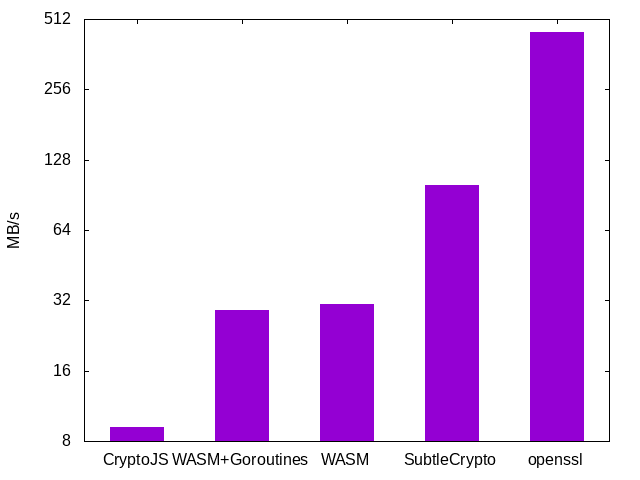
\includegraphics[width=0.7\linewidth]{images/hashingperformance.png}
        \caption{Time in seconds for hashing 1GB of random data}
        \label{fig:hashingperformance}
    \end{center}
\end{figure}


\subsection{Deciding On The In-Browser Hashing Implementation}
\label{subsec:deciding-on-the-in-browser-hashing-implementation}
It is clear from figure~\ref{fig:hashingperformance} that CryptoJS is significantly faster than the other options we tried.
Given that it supports piece-wise hashing as well,
something we need for larger files (as discussed in section~\ref{subsec:browserhashing}), the choice is clear.
We will use CryptoJS to hash the input files in the browser.














    %---------------------------------------------------------------------------

    % Selbständigkeitserklärung
    %---------------------------------------------------------------------------
    \cleardoublepage
    \phantomsection
    \addcontentsline{toc}{chapter}{Declaration of authorship}
    \chapter*{Declaration of primary authorship}
\label{chap:declaration_authorship}

\vspace*{10mm} 

I / We hereby confirm that I / we have written this thesis independently and without using other sources and resources than those specified in the bibliography. All text passages which were not written by me are marked as quotations and provided with the exact indication of its origin. 

\vspace{15mm}

\begin{tabbing}
xxxxxxxxxxxxxxxxxxxxxxxxxxxxxx\=xxxxxxxxxxxxxxxxxxxxxxxxxxxxxx\=xxxxxxxxxxxxxxxxxxxxxxxxxxxxxx\kill
Place, Date:		\> [Biel/Burgdorf], \versiondate \\ \\ 
Last Name/s, First Name/s:	\> [Test Peter] 	\> [M\"uster R\"os\"a] \\ \\ \\ \\ 
Signature/s:	\> ......................................\> ...................................... \\
\end{tabbing}

    %---------------------------------------------------------------------------

    % Glossary
    %---------------------------------------------------------------------------
    \cleardoublepage
    \phantomsection
    \addcontentsline{toc}{chapter}{Glossay}
    %\renewcommand{\glossaryname}{Glossay}
    \printglossary
    %---------------------------------------------------------------------------

    % Bibliography
    %---------------------------------------------------------------------------
    \cleardoublepage
    \phantomsection
    \addcontentsline{toc}{chapter}{Bibliography}
    \bibliographystyle{IEEEtranS}
    \bibliography{database/bibliography}{}
    %---------------------------------------------------------------------------

    % Listings
    %---------------------------------------------------------------------------
    \cleardoublepage
    \phantomsection
    \addcontentsline{toc}{chapter}{List of figures}
    \listoffigures
    \cleardoublepage
    \phantomsection
    \addcontentsline{toc}{chapter}{List fo tables}
    \listoftables
    %---------------------------------------------------------------------------

    % Index
    %---------------------------------------------------------------------------
    \cleardoublepage
    \phantomsection
    \addcontentsline{toc}{chapter}{Index}
    \printindex
    %---------------------------------------------------------------------------

    % Attachment:
    %---------------------------------------------------------------------------
    \appendix
    \settocdepth{section}
%    \chapter*{APPENDICES}
\addcontentsline{toc}{chapter}{APPENDICES}

\begingroup\let\clearpage\relax
\chapter{Arbitrary Appendix}
\label{chap:appendix_arb}
\endgroup

The European languages are members of the same family. Their separate existence is a myth. For science, music, sport, etc, Europe uses the same vocabulary. The languages only differ in their grammar, their pronunciation and their most common words. Everyone realizes why a new common language would be desirable: one could refuse to pay expensive translators. To achieve this, it would be necessary to have uniform grammar, pronunciation and more common words. If several languages coalesce, the grammar of the resulting language is more simple and regular than that of the individual languages. The new common language will be more simple and regular than the existing European languages. It will be as simple as Occidental; in fact, it will be Occidental. 
%    \chapter{Additional Appendix}
\label{chap:appendix_B}

\section{Test 1}
To an English person, it will seem like simplified English, as a skeptical Cambridge friend of mine told me what Occidental is. The European languages are members of the same family. Their separate existence is a myth. For science, music, sport, etc, Europe uses the same vocabulary. The languages only differ in their grammar, their pronunciation and their most common words. Everyone realizes why a new common language would be desirable: one could refuse to pay expensive translators. To achieve this, it would be necessary to have uniform grammar, pronunciation and more common words. If several languages coalesce, the grammar of the resulting language is more simple and regular than that of the individual languages. The new common language will be more simple and regular than the existing European languages. 

\subsection{Environment}
It will be as simple as Occidental; in fact, it will be Occidental. To an English person, it will seem like simplified English, as a skeptical Cambridge friend of mine told me what Occidental is. The European languages are members of the same family. Their separate existence is a myth. For science, music, sport, etc, Europe uses the same vocabulary. The languages only differ in their grammar, their pronunciation and their most common words. Everyone realizes why a new common language would be desirable: one could refuse to pay expensive translators. To achieve this, it would be necessary to have uniform grammar, pronunciation and more common words.
%    \chapter{Content of CD-ROM}
\label{chap:appendix_CDROM}

Content of the enclosed CD-ROM, directory tree, etc.
    %---------------------------------------------------------------------------

    %---------------------------------------------------------------------------
\end{document}

